% !TeX root = ../tcc.tex
\chapter{Revisão sistemática da literatura}
\label{cap:revisao-literatura}
\label{sec:conducao-revisao}

A revisão de literatura foi planejada para identificar e analisar evidências
sobre a avaliação de modelos de visão computacional aplicados a manifestações
cutâneas associadas à hanseníase. A definição de uma questão, de um protocolo,
de critérios de seleção e de procedimentos de extração e síntese é coerente
com as orientações de \citeonline{kitchenham2007} para revisões sistemáticas
em engenharia de software. O capítulo 4 de \citeonline[p. 51--56]{wohlin2024} apresenta a revisão
sistemática como estudo secundário e organiza seu processo em planejamento,
condução e relato. A obra fundamenta a definição de questões e critérios,
a documentação da busca, a seleção e a extração orientada pelas questões
de pesquisa. O procedimento
adotado nesta revisão é descrito a seguir; suas etapas não devem ser
interpretadas como a execução de um experimento controlado.

\section{Planejamento e protocolo}

O objetivo, o protocolo e os critérios foram organizados no Evidentia. A
questão principal é: como avaliar o desempenho de modelos de visão
computacional aplicados à identificação de padrões associados à hanseníase
em imagens de pele, no contexto da rede pública de saúde do Brasil?

As questões secundárias desdobram a questão principal em aspectos necessários
à avaliação dos modelos: técnicas e abordagens utilizadas, dados e populações,
procedimentos, métricas, desempenho entre grupos e generalização. A
identificação dos veículos de publicação complementa a caracterização dos
estudos. Conforme \citeonline{kitchenham2007}, as questões de pesquisa
orientam a definição dos dados a serem extraídos e sintetizados na revisão. A
investigação foi detalhada nas seguintes questões secundárias:

\begin{enumerate}
\item Quais técnicas de visão computacional são usadas para identificar manifestações dermatológicas associadas à hanseníase?
\item Quais conjuntos de dados e populações são utilizados no desenvolvimento e na avaliação dos modelos?
\item Quais métodos e procedimentos são usados para avaliar o desempenho e quais resultados são relatados?
\item Quais métricas são usadas na avaliação e quais resultados são relatados?
\item Como o desempenho varia entre diferentes grupos ou tons de pele?
\item Quais modelos e abordagens de inteligência artificial são utilizados para identificar as manifestações dermatológicas associadas à doença?
\item Como a capacidade de generalização é avaliada, especialmente em conjuntos diferentes dos usados no treinamento?
\item Em que tipo de veículo o artigo foi publicado, como periódico ou conferência?
\end{enumerate}

\section{Estruturação da estratégia de busca}

Para estruturar a solicitação de busca, foram utilizados os componentes
registrados como população, contexto, intervenção e resultado do PICOC.
A população foi representada por termos de visão computacional,
inteligência artificial, redes neurais e aprendizado de máquina e profundo;
o contexto, por hanseníase e classificação ou segmentação de lesões
cutâneas; a intervenção, por modelos e arquiteturas de aprendizado de
máquina; e o resultado, por termos de avaliação, métricas e tarefas de
identificação. O \textit{prompt} preservado não apresenta um campo
separado de comparação. As perguntas e a relação completa de termos,
incluindo sinônimos e asteriscos, foram consolidadas no \textit{prompt}
estruturado submetido à plataforma Consensus, apresentado na
Subseção~\ref{subsec:prompt-consensus} (Quadro~\ref{qua:prompt-consensus}).

A Figura~\ref{fig:pico-pai} apresenta a representação PICO de
\citeonline{pai2004}, originalmente voltada à formulação de questões
clínicas. Nela, \textit{patient}, \textit{intervention}, \textit{comparison}
e \textit{outcome} correspondem, respectivamente, a paciente ou população,
intervenção, comparação e resultado. O PICOC acrescenta o contexto a esses
componentes. No procedimento deste trabalho, o \textit{prompt} utilizou
população, intervenção, contexto e resultado, sem campo específico de
comparação; a figura apresenta o modelo conceitual PICO e não afirma que
uma busca booleana exatamente igual à ilustrada foi executada.

\begin{figure}[htbp]
\centering
\caption{Representação dos componentes PICO para uma estratégia de busca}
\label{fig:pico-pai}
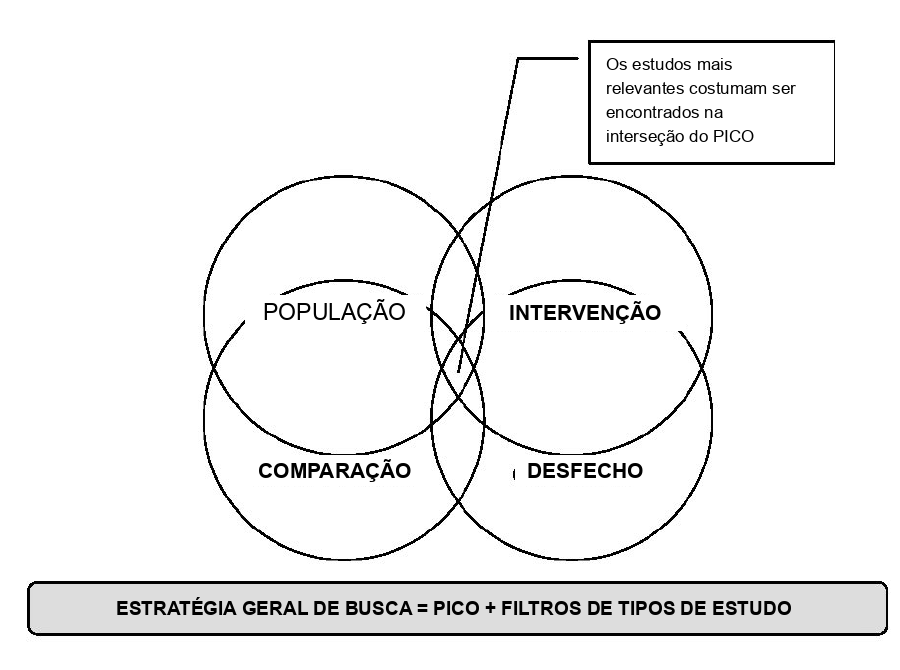
\includegraphics[width=0.68\textwidth]{figuras/pico-pai-2004.png}
\fonte{Reproduzido de \citeonline[p. 89, Figura 3]{pai2004}.}
\end{figure}

\subsection{Definição dos componentes PICOC e string de busca}
\label{subsec:picoc-string-busca}

A formulação da estratégia de busca orientou-se pela adaptação dos elementos do modelo PICOC (\textit{Population, Intervention, Comparison, Outcome, Context}) \cite{pai2004,kitchenham2007}, permitindo delimitar termos centrais e sinônimos relevantes para recuperar estudos que investigam a aplicação de visão computacional e inteligência artificial no diagnóstico da hanseníase. A Tabela~\ref{tab:picoc-termos} detalha os termos centrais e os operadores de expansão semântica definidos para cada faceta do protocolo.

\begin{table}[htb]
\centering
\caption{Componentes do modelo PICOC adaptado e termos de busca}
\label{tab:picoc-termos}
\small
\begin{tabular}{p{2.6cm} p{3.0cm} p{8.4cm}}
\toprule
\textbf{Elemento} & \textbf{Termo Central} & \textbf{Sinônimos e Termos Relacionados} \\
\midrule
\textbf{População} & \textit{Computer Vision} / IA & \textit{artificial intelligence}, \textit{CNN}, \textit{convolutional neural network*}, \textit{deep learning}, \textit{machine learning}, \textit{neural network*} \\
\textbf{Intervenção} & Modelos de Aprendizado & \textit{ResNet*}, \textit{DenseNet*}, \textit{EfficientNet*}, \textit{U-Net}, \textit{UNet}, \textit{Attention U-Net}, \textit{Vision Transformer*}, \textit{ViT}, \textit{ConvNeXt*}, \textit{Swin Transformer*}, \textit{transfer learning}, \textit{supervised learning} \\
\textbf{Contexto} & Hanseníase & \textit{leprosy}, \textit{Hansen disease}, \textit{Hansen's disease}, \textit{hanseniasis}, \textit{skin lesion classification}, \textit{skin lesion segmentation} \\
\textbf{Desfecho} (\textit{Outcome}) & Desempenho e Métricas & \textit{accuracy}, \textit{AUC}, \textit{ROC-AUC}, \textit{sensitivity}, \textit{specificity}, \textit{precision}, \textit{recall}, \textit{F1-score}, \textit{detection}, \textit{diagnosis}, \textit{evaluation}, \textit{segmentation} \\
\bottomrule
\end{tabular}
\fonte{Autores.}
\end{table}

A partir do mapeamento dos componentes, a string de busca foi estruturada aplicando o operador lógico booleano \texttt{OR} entre os termos e sinônimos no interior de cada dimensão temática, e o operador booleano \texttt{AND} para conectar as quatro facetas fundamentais do protocolo (\textit{População} \texttt{AND} \textit{Intervenção} \texttt{AND} \textit{Contexto} \texttt{AND} \textit{Desfecho}). A consulta booleana estruturada é apresentada a seguir:

\begin{center}
\fbox{
\begin{minipage}{0.94\textwidth}
\footnotesize\ttfamily
( "Computer Vision" OR "artificial intelligence" OR "CNN" OR "convolutional neural network*" OR "deep learning" OR "machine learning" OR "neural network*" ) \\
\textbf{AND} \\
( "leprosy" OR "Hansen disease" OR "Hansen's disease" OR "hanseniasis" OR "skin lesion classification" OR "skin lesion segmentation" ) \\
\textbf{AND} \\
( "ResNet*" OR "DenseNet*" OR "EfficientNet*" OR "U-Net" OR "UNet" OR "Vision Transformer*" OR "ViT" OR "transfer learning" OR "supervised learning" OR "Few-shot" ) \\
\textbf{AND} \\
( "accuracy" OR "AUC" OR "sensitivity" OR "specificity" OR "precision" OR "recall" OR "F1-score" OR "ROC-AUC" OR "evaluation" OR "detection" OR "segmentation" )
\end{minipage}
}
\end{center}

\subsection{Prompt estruturado submetido à plataforma Consensus}
\label{subsec:prompt-consensus}

Diferentemente dos motores de busca acadêmicos convencionais baseados exclusivamente na correspondência estrita de operadores booleanos, a plataforma Consensus emprega inteligência artificial para recuperação semântica em grafos de citações e literatura biomédica. Por essa razão, a formulação submetida à ferramenta integrou a questão norteadora principal, as oito perguntas secundárias da revisão e a totalidade dos termos e sinônimos delimitados na matriz PICOC em um \textit{prompt} estruturado em língua inglesa.

O Quadro~\ref{qua:prompt-consensus} reproduz integralmente a solicitação submetida à plataforma Consensus, preservando a sintaxe original, a estrutura das facetas conceituais e os operadores de truncamento aplicados aos termos técnicos.

\lstinputlisting[
  caption={Prompt estruturado em linguagem natural submetido à plataforma Consensus},
  label={qua:prompt-consensus},
  basicstyle=\scriptsize\ttfamily,
  breaklines=true,
  breakatwhitespace=true,
  columns=flexible,
  keepspaces=true,
  frame=single,
  rulecolor=\color{black!30},
  backgroundcolor=\color{black!2},
  xleftmargin=0.5em,
  xrightmargin=0.5em
]{editaveis/prompt-consensus.txt}
\vspace{-0.2cm}\noindent\footnotesize\textbf{Fonte:} Autores.\vspace{0.4cm}

\subsection{Consultas apresentadas pelo Consensus}

Na busca de 25 de setembro de 2026, o Consensus apresentou uma sequência
de consultas em quatro rodadas. A Tabela~\ref{tab:consultas-consensus}
reproduz os textos e indicadores exibidos. Esses indicadores são saídas
internas da ferramenta, sem definição operacional disponível; não
correspondem a contagens auditadas de estudos únicos triados pela dupla.

\begin{longtable}{p{0.08\textwidth}p{0.68\textwidth}r}
\caption{Consultas e indicadores apresentados pelo Consensus}\label{tab:consultas-consensus}\\
\toprule
Rodada & Consulta & Indicador \\
\midrule
\endfirsthead
\toprule Rodada & Consulta & Indicador \\
\midrule
\endhead
1 & deep learning convolutional neural network leprosy Hansen disease skin lesion classification detection diagnosis & 95,3 mil \\
1 & U-Net ResNet EfficientNet Vision Transformer skin lesion segmentation leprosy hanseniasis dermatological pattern recognition & 2,3 mil \\
1 & machine learning model performance evaluation accuracy AUC F1 sensitivity specificity leprosy skin image diagnosis & 63,5 mil \\
1 & skin tone fairness demographic subgroup performance dermatology AI model external validation generalization cross-dataset & 67,4 mil \\
2 & leprosy skin image dataset Brazil public health AI diagnosis computer vision & 26,2 mil \\
2 & transfer learning self-supervised semi-supervised learning skin neglected tropical disease leprosy image classification & 36,6 mil \\
2 & WHO skin neglected tropical diseases mobile application telemedicine leprosy detection low-resource settings & 63,4 mil \\
3 & explainability XAI Grad-CAM interpretable AI leprosy neglected tropical disease skin lesion diagnosis & 1,6 mil \\
3 & histopathological image analysis acid-fast bacilli detection deep learning leprosy nerve biopsy microscopy & 17,6 mil \\
4 & leprosy skin image dataset multimodal clinical metadata paucibacillary multibacillary classification AI model & 3 mil \\
4 & reporting standards quality assessment QUADAS CONSORT-AI CLEAR dermatology AI model evaluation systematic review & 47,8 mil \\
\bottomrule
\end{longtable}

O painel informou ainda os indicadores \textit{Retrieved} de 425,4 mil,
\textit{Eligible} de mil e \textit{Included} de 100. Após a segunda
rodada, a ferramenta apresentou uma expansão por grafo de citações com dez
sementes e o indicador 662; após a terceira, indicou leitura de 12
resumos; antes da síntese, indicou leitura de resumos e PDFs de 100 itens.
O significado operacional desses indicadores, a identificação completa
das sementes e o acesso integral a cada PDF não foram comprovados. A
busca também foi ampliada para temas relacionados, como dermatologia geral,
equidade, saúde móvel, microscopia, histopatologia e diretrizes de relato;
nessas condições, a presença de uma referência na saída da ferramenta não
significa que ela atende aos critérios da revisão.


\section{Realização da busca e seleção dos artigos}
\label{sec:execucao-busca-selecao}

Para conferir rigor metodológico, reprodutibilidade e transparência à revisão sistemática da literatura, o processo de identificação, deduplicação, triagem por título e resumo, avaliação de elegibilidade e extração foi conduzido por meio de um fluxo de trabalho assistido por ferramentas de inteligência artificial especializadas, articuladas sob contínuo julgamento crítico e validação por pares da dupla de pesquisadores.

A Figura~\ref{fig:fluxo-metodologico-ia} ilustra o fluxo metodológico integrado, evidenciando as seis etapas da revisão, os volumes documentais em cada transição e a atuação específica de cada ferramenta de apoio (\textit{Consensus}, \textit{Claude}, \textit{JevReviewer} e \textit{Evidentia Review}).

\begin{figure}[htbp]
\centering
\begin{tikzpicture}[
  stage/.style={
    draw=black!75,
    fill=white,
    thick,
    rounded corners=3pt,
    text width=6.4cm,
    font=\small,
    inner sep=6pt
  },
  tool/.style={
    draw=black!30,
    fill=blue!5,
    rounded corners=2pt,
    text width=5.2cm,
    font=\scriptsize,
    inner sep=5pt
  },
  excl/.style={
    draw=red!70,
    fill=red!5,
    rounded corners=2pt,
    text width=5.2cm,
    font=\scriptsize,
    inner sep=5pt
  },
  finalstage/.style={
    draw=black!75,
    fill=blue!8,
    line width=1.1pt,
    rounded corners=3pt,
    text width=6.4cm,
    font=\small,
    inner sep=6pt
  },
  mainarrow/.style={
    -{Stealth[length=2.5mm]},
    line width=1.2pt,
    draw=black!80
  },
  conn/.style={
    -{Stealth[length=1.8mm]},
    draw=black!60,
    dashed,
    thick
  }
]

% 1. Protocolo
\node[stage] (s1) {\textbf{1. Planejamento e Protocolo}\\
\footnotesize Definição da questão principal, 8 RQs secundárias, matriz PICOC e critérios de elegibilidade (CI01--05 e CE01--05).};

\node[tool, right=0.6cm of s1] (t1) {\textbf{Evidentia Review} (\textit{Gestão})\\
Cadastro estruturado do protocolo, formulários de extração e governança do processo.};

% Headers
\node[font=\bfseries\small, above=0.25cm of s1] (h1) {Etapas Metodológicas da RSL};
\node[font=\bfseries\small, above=0.25cm of t1] (h2) {Ferramentas de IA e Desdobramentos};

% 2. Busca e Identificação
\node[stage, below=0.45cm of s1] (s2) {\textbf{2. Busca e Identificação Inicial}\\
\footnotesize Execução de buscas especializadas com prompt semântico estruturado em língua inglesa.};

\node[tool] (t2) at (s2 -| t1) {\textbf{Consensus} (100 reg., 98 com DOI)\\
$\rightarrow$ Busca semântica e grafo biomédico\\
\textbf{Claude} (30 reg. complementares)\\
\textbf{Total Bruto: 130 registros}};

% 3. Deduplicação
\node[stage, below=0.45cm of s2] (s3) {\textbf{3. Deduplicação e Pré-Triagem}\\
\footnotesize Resolução de redundâncias bibliográficas via cruzamento automatizado por DOI e títulos.};

\node[excl] (t3) at (s3 -| t1) {\textbf{12 duplicatas removidas}\\
\textit{Aplicação do critério CE01 (Duplicatas)}\\
$\rightarrow$ Restam \textbf{118 registros únicos} para triagem.};

% 4. Triagem Título/Resumo
\node[stage, below=0.45cm of s3] (s4) {\textbf{4. Triagem por Título e Resumo}\\
\footnotesize Avaliação preditiva acelerada por IA associada ao julgamento crítico por pares da dupla.};

\node[tool] (t4) at (s4 -| t1) {\textbf{JevReviewer}: predição e 5 \textit{fail scores}\\
\textbf{Evidentia Review} (decisão por pares):\\
$\bullet$ 91 excluídos \quad $\bullet$ 1 intermediário\\
$\bullet$ \textbf{26 selecionados para texto integral}};

% 5. Leitura na Íntegra
\node[stage, below=0.45cm of s4] (s5) {\textbf{5. Avaliação de Elegibilidade}\\
\footnotesize Leitura minuciosa de 26 artigos integrais e checagem de conformidade com os critérios.};

\node[excl] (t5) at (s5 -| t1) {\textbf{1 estudo excluído}\\
\textit{Aplicação do critério CE04 (GenAI exclusiva)}\\
$\rightarrow$ Joerg et al. (2025): dados puramente sintéticos, sem pacientes ou imagens clínicas.};

% 6. Extração e Síntese
\node[finalstage, below=0.45cm of s5] (s6) {\textbf{6. Extração Padronizada e Síntese}\\
\footnotesize Preenchimento estruturado de \textbf{18 campos padronizados} sobre os \textbf{25 estudos definitivos}.};

\node[tool, draw=green!60!black, fill=green!6] (t6) at (s6 -| t1) {\textbf{Evidentia Review \& Síntese Final}\\
Matriz de dados consolidada:\\
$\bullet$ Extração de modelos, métricas e fototipos\\
$\bullet$ Respostas aprofundadas para RQ1 a RQ8};

% Downward main arrows
\draw[mainarrow] (s1) -- (s2);
\draw[mainarrow] (s2) -- (s3);
\draw[mainarrow] (s3) -- (s4);
\draw[mainarrow] (s4) -- (s5);
\draw[mainarrow] (s5) -- (s6);

% Horizontal connections
\draw[conn] (t1) -- (s1);
\draw[conn] (t2) -- (s2);
\draw[conn] (s3) -- (t3);
\draw[conn] (t4) -- (s4);
\draw[conn] (s5) -- (t5);
\draw[conn] (t6) -- (s6);

\end{tikzpicture}
\caption{Fluxo metodológico da Revisão Sistemática da Literatura assistido por ferramentas de inteligência artificial}
\label{fig:fluxo-metodologico-ia}
\fonte{Autores.}
\end{figure}

\subsection{Busca e identificação dos registros}

O protocolo da revisão foi organizado no Evidentia a partir da questão de
pesquisa e dos componentes do PICOC. Esses elementos foram utilizados em
uma solicitação em inglês ao Consensus, sem a inclusão dos critérios de
seleção no texto do \textit{prompt}. Em 25 de setembro de 2026, a
ferramenta retornou uma lista de 100 referências, das quais 98 tinham DOI
informado. Foi registrada também uma busca complementar por meio do Claude, da qual
foram reunidas 30 referências. A data, o \textit{prompt}, o modelo, a configuração e a lista completa
dessa busca complementar ainda precisam ser confirmados. Embora o protocolo
também registre a Scopus como fonte, não há comprovação de uma busca separada
nessa base na etapa descrita.

As duas listas somaram 130 registros e,
após a remoção de duplicatas, permaneceram 118 para triagem. A diferença
entre esses totais corresponde a 12 registros removidos; entretanto, os
pares considerados duplicados e o procedimento usado para identificá-los
ainda não foram integralmente documentados. O conjunto bibliográfico disponível contém 129 entradas. Na comparação
com os 118 registros triados, onze entradas não aparecem no conjunto de triagem e apresentam o mesmo DOI de outras entradas nele
representadas. Essa comparação permite identificar 11 pares de
registros com DOI coincidente, mas não identifica um eventual décimo
segundo registro removido nem comprova, isoladamente, quando cada par
foi deduplicado. A diferença entre as 129 entradas identificadas e os
130 registros informados no relato permanece a esclarecer. Os
indicadores internos apresentados pelo Consensus não foram tratados
como quantidades auditadas de estudos únicos examinados pelos pesquisadores.

\subsection{Critérios de seleção}

Os critérios de inclusão foram: disponibilidade do texto completo (CI01);
uso de visão computacional, aprendizado de máquina ou aprendizado profundo
para detectar, classificar, identificar ou segmentar manifestações
cutâneas humanas associadas à hanseníase (CI02); relato ou síntese de
evidências de avaliação de métodos de inteligência artificial para
hanseníase, incluindo experimentos, testes, validação ou comparação de
desempenho (CI03); uso, análise ou revisão de fotografias clínicas ou
imagens dermatoscópicas de lesões cutâneas humanas associadas à hanseníase
(CI04); e inclusão da hanseníase entre as condições avaliadas em trabalhos
que abordam múltiplas doenças (CI05). A formulação preservada do CI03 foi
recebida truncada após ``resultados de estu''; o trecho descrito acima
resume apenas a parte legível e sua redação integral deve ser confirmada.
Os critérios abrangem estudos primários e revisões, que devem ser
distinguidos durante a extração.

Foram informados os seguintes critérios de exclusão: registro duplicado de
artigo já considerado (CE01); publicação anterior a 2020 (CE02); texto
completo em idioma diferente de inglês ou português (CE03); uso exclusivo
de inteligência artificial generativa como intervenção (CE04); e ausência
de abordagem da hanseníase (CE05). A verificação de disponibilidade e
idioma do texto completo pode depender de consulta além do título e do
resumo, enquanto data e duplicidade também dependem dos metadados.

\subsection{Triagem e seleção para leitura integral}

O Jev Reviewer foi utilizado como apoio à classificação preliminar dos
118 registros. Para cada registro, suas sugestões são acompanhadas de
valores associados ao não atendimento de cinco critérios:
\begin{enumerate}
\item Abordar a hanseníase como condição investigada ou avaliada,
isoladamente ou entre outras doenças; uma menção apenas introdutória não
atende a esse critério.
\item Utilizar fotografias clínicas ou imagens dermatoscópicas de
manifestações cutâneas humanas associadas à hanseníase, ou revisar estudos
que utilizam essas imagens.
\item Aplicar ou analisar métodos de visão computacional, aprendizado de
máquina ou aprendizado profundo para detectar, classificar, identificar
ou segmentar essas manifestações nas imagens, incluindo revisões dessas
aplicações.
\item Relatar ou sintetizar evidências de avaliação desses métodos, como
experimentos, testes, validação, comparação de desempenho ou resultados
de estudos.
\item Não se limitar exclusivamente à inteligência artificial generativa
como intervenção.
\end{enumerate}

Esses cinco critérios descrevem o que foi avaliado pelo Jev; eles não
substituem os critérios gerais de inclusão e exclusão da revisão. Os valores
de \texttt{fails} acompanham a avaliação automatizada e não registram, por
si sós, a justificativa da decisão dos pesquisadores. Após a classificação
preliminar, a dupla relatou ter revisado os registros por título e resumo,
com as decisões registradas no Evidentia. A documentação não esclarece se
ambos avaliaram todos os registros de maneira independente. A avaliação por
dois ou mais pesquisadores, ao menos para uma amostra, é recomendada por
\citeonline[p. 55]{wohlin2024}; essa recomendação não demonstra que ela
foi executada neste trabalho.

As sugestões do Jev para os 118 registros foram: duas de inclusão, 15 incertas e 101 de exclusão.
O cruzamento por título entre as sugestões e as decisões do Evidentia
identificou correspondência para todos os registros. Entre os 26 com
situação de inclusão no Evidentia, dois tinham sugestão de inclusão do
Jev, 11 tinham sugestão incerta e 13 tinham sugestão de exclusão. Entre
os 91 excluídos no Evidentia, 87 tinham sugestão de exclusão e quatro
tinham sugestão incerta. O registro restante, classificado como
intermediário no Evidentia, tinha sugestão de exclusão pelo Jev. Assim,
as sugestões automáticas são distintas das decisões de triagem. A data de
execução, o modelo, a configuração completa e a versão da ferramenta não
foram identificados; os cinco critérios exibidos acima, por sua vez, estão
registrados nas avaliações disponíveis.

Os estados intermediários da triagem registram, em uma etapa, 12 inclusões,
32 exclusões, 15 decisões intermediárias e 59 registros sem decisão. Em
outro estado foram observadas 19 inclusões, 40 exclusões e os mesmos 59
registros sem decisão; as 15 decisões intermediárias passaram a sete
inclusões e oito exclusões. As datas das decisões preenchidas indicam
28 de setembro de 2026, mas não registram horário de cada decisão. Esses
estados intermediários não devem ser confundidos com o resultado
consolidado descrito a seguir.

No Evidentia, 91 registros apresentam decisão de exclusão,
26 de inclusão e uma decisão intermediária, totalizando 118 registros.
Esse último registro, \textit{Leprosy Screening Based on Artificial
Intelligence: Development of a Cross-Platform App} \cite{souza2021}, apresenta duas
decisões individuais de exclusão, mas sua decisão consolidada foi
registrada manualmente como intermediária. Em outro registro,
\textit{Leprosy lesion recognition using convolutional neural networks} \cite{baweja2016},
houve uma decisão individual de inclusão e uma de exclusão; o conflito
foi resolvido manualmente com decisão consolidada de exclusão. Os demais
116 registros possuem decisão consolidada automática, segundo o campo
correspondente no Evidentia. Essa classificação descreve o mecanismo de
consolidação registrado pelo sistema e não identifica uma revisão
independente por ambos os pesquisadores para cada artigo.

A decomposição 91 exclusões, 26 inclusões e uma decisão intermediária
esclarece a diferença observada no registro anterior: 118 menos 26 é 92,
mas esse resultado reúne os 91 excluídos e o registro intermediário.
Assim, não se deve representar a diferença de 92 como 92 exclusões.
Os 26 registros com situação de inclusão na triagem constituíram o conjunto
encaminhado à leitura integral. Após a análise aprofundada dos textos completos e
verificação dos critérios de elegibilidade no formulário de extração, 25 estudos foram
confirmados e integralmente extraídos. O registro divergente \cite{joerg2025} foi excluído
da síntese qualitativa final por avaliar unicamente imagens dermatológicas sintéticas
geradas por inteligência artificial generativa, sem envolver pacientes reais ou dados clínicos de hanseníase.

A Figura~\ref{fig:fluxo-triagem} sintetiza as quantidades descritas nesta
seção. A indicação de 12 registros removidos corresponde à diferença entre
130 e 118, decorrente da deduplicação das fontes de identificação. O processo
culminou na seleção definitiva de 25 estudos para extração e síntese.

\begin{figure}[htbp]
\centering
\caption{Fluxo de identificação, triagem e inclusão dos estudos}
\label{fig:fluxo-triagem}
\begin{tikzpicture}[
  box/.style={draw,rounded corners=2pt,align=center,text width=3.6cm,minimum height=1.0cm,inner sep=5pt,font=\small},
  wide/.style={box,text width=7.6cm},
  arrow/.style={-{Stealth[length=2.3mm]},thick}
]
\node[wide] (identified) {Registros informados: 130\\(Consensus: 100; Claude: 30)};
\node[wide,below=1.5cm of identified] (screened) {Registros após deduplicação: 118\\para triagem por título e resumo};
\draw[arrow] (identified) -- node[right=3mm,align=left,font=\scriptsize,text width=4cm] {12 registros removidos\\(duplicatas / pré-triagem)} (screened);
\node[box,below=1.15cm of screened,xshift=-4.3cm] (excluded) {Excluídos\\91 registros};
\node[box,below=1.15cm of screened] (included) {Incluídos na triagem\\26 registros};
\node[box,below=1.15cm of screened,xshift=4.3cm] (maybe) {Decisão\\intermediária\\1 registro};
\draw[arrow] (screened.south) -- ++(0,-0.45) -| (excluded.north);
\draw[arrow] (screened.south) -- (included.north);
\draw[arrow] (screened.south) -- ++(0,-0.45) -| (maybe.north);
\node[box,below=0.85cm of included] (fulltext) {Leitura integral e extração\\25 estudos incluídos\\(1 excluído: sintético)};
\draw[arrow] (included) -- (fulltext);
\end{tikzpicture}
\fonte{Autores.}
\end{figure}

\begin{table}[htb]
\centering
\caption{Quantidades documentadas na identificação, triagem e inclusão dos estudos}
\label{tab:fluxo-selecao-estudos}
\begin{tabular}{p{0.66\textwidth} r}
\toprule
Etapa ou registro & Quantidade \\
\midrule
Referências informadas do Consensus & 100 \\
Referências informadas do Claude & 30 \\
Registros reunidos & 130 \\
Registros removidos na pré-triagem (duplicatas) & 12 \\
Registros submetidos à triagem no Evidentia & 118 \\
Excluídos na triagem por título e resumo & 91 \\
Incluídos na triagem para leitura integral & 26 \\
Decisão intermediária (avaliada e resolvida) & 1 \\
Excluído após leitura integral (escopo sintético de imagem) & 1 \\
Estudos incluídos definitivamente com extração completa & 25 \\
\bottomrule
\end{tabular}
\fonte{Autores.}
\end{table}

O formulário de extração no sistema Evidentia reúne os 25 estudos incluídos
definitivamente após a leitura integral e verificação de elegibilidade, com todos os seus
18 campos padronizados integralmente preenchidos. Entre os 26 registros pré-selecionados na
triagem, o estudo \textit{AI-generated dermatologic images show deficient skin tone
diversity and poor diagnostic accuracy: An experimental study} \cite{joerg2025} não
integrou a extração final por investigar exclusivamente a geração de imagens sintéticas
por difusão estável e avaliar disparidades fenotípicas teóricas em dermatologia geral,
sem envolver conjuntos de dados clínicos de pacientes acometidos por hanseníase.

Para assegurar a rastreabilidade do processo de seleção, os motivos de exclusão dos 91
registros descartados na fase de triagem foram catalogados com base nas violações aos
critérios de elegibilidade (estudos fora do escopo de visão computacional, doenças não
relacionadas ou resumos inconclusivos). Com a resolução das divergências e a conclusão
da leitura aprofundada, consolidou-se o conjunto definitivo de 25 estudos que subsidiam
as análises empíricas desta monografia.

\subsection{Extração e síntese das evidências}

Conforme \citeonline[p. 55--56]{wohlin2024}, o formulário de extração
deve ser orientado pelas questões de pesquisa e permitir o registro das
características dos estudos e dos dados necessários à síntese. Neste
trabalho, o formulário foi organizado para registrar título, autores,
ano, fonte, tipo de estudo e veículo, além das respostas detalhadas às questões da
revisão: técnicas de visão computacional, bases de dados, características das populações, manifestações cutâneas, quantidade de
imagens, métodos e procedimentos de avaliação, métricas, resultados obtidos, informações sobre tons de pele,
modelos de inteligência artificial, avaliação de generalização, métodos de validação e limitações relatadas. A extração completa dos 25 estudos permitiu correlacionar sistematicamente cada achado com as páginas e tabelas de origem, distinguindo rigorosamente estudos primários e revisões para evitar atribuições indevidas de métricas secundárias.

A síntese apresentada a seguir distingue formalmente as tarefas de classificação diagnóstica, detecção e segmentação de feridas, bem
como compara os desempenhos globais multiclasse com os resultados específicos obtidos para hanseníase. As lacunas documentadas a respeito da ausência de estratificação por tons de pele e as limitações de validação externa em bases independentes evidenciam a relevância científica do tema e balizam a discussão sobre a viabilidade e os riscos de implantação dessas ferramentas no SUS.

\section{Resultados da revisão}
\label{sec:resultados-revisao}

Esta seção apresenta a síntese qualitativa e quantitativa das evidências
extraídas dos 25 estudos primários e secundários incluídos definitivamente
na revisão sistemática da literatura. Os dados foram extraídos a partir de
formulário estruturado no Evidentia Review, composto por 18 campos padronizados,
permitindo responder detalhadamente a cada uma das questões secundárias de
pesquisa estabelecidas no protocolo.

\subsection{Quais técnicas de visão computacional são utilizadas?}
\label{subsec:rq1-tecnicas}

A análise dos 25 estudos incluídos demonstra que as técnicas de visão computacional
empregadas no contexto da hanseníase organizam-se ao longo de quatro etapas principais
do fluxo de processamento de imagens: pré-processamento, delimitação de regiões de
interesse (segmentação), extração de atributos para classificação e explicabilidade visual.

No pré-processamento, identifica-se o predomínio de operações voltadas à atenuação
da variabilidade de captura fotográfica em cenários ambulatoriais e comunitários.
Destacam-se o redimensionamento padronizado (comumente para matrizes de $224 \times 224$
pixels em conformidade com as entradas de redes convolucionais pré-treinadas no ImageNet
\cite{yotsu2026}), equalização de contraste, filtragem adaptativa de ruídos e
conversão para escala de cinza acompanhada de limiarização adaptativa de Otsu
\cite{barbieri2022,mehta2026}. Observa-se ainda o recurso frequente ao recorte manual
da lesão (\textit{cropping}) e à anonimização por mascaramento seletivo \cite{deps2026,sadanand2023}.

Para a tarefa de segmentação, a literatura divide-se entre abordagens semânticas profundas
e métodos heurísticos clássicos. Enquanto estudos de feridas crônicas e sequelas neuropáticas
utilizam arquiteturas baseadas em U-Net, DeepLabV3+ e SegNet para mapear bordas e classificar
tecidos de granulação, esfacelo e necrose \cite{sanchez2024,mehta2026}, trabalhos voltados
a lesões cutâneas ativas empregam agrupamento por \textit{Fuzzy C-Means} otimizado por
algoritmos bioinspirados (\textit{Firefly Algorithm} e otimização por enxame de partículas)
\cite{jitendra2024heuristic} associados a operações morfológicas de dilatação e erosão.

Na etapa de extração e classificação, coexistem métodos tradicionais e modelos profundos.
Estudos exploratórios aplicam descritores manuais de textura, como \textit{Local Binary Patterns}
(LBP) e \textit{Weber Local Descriptor} (WLD) fusionados a classificadores supervisionados
(SVM e Random Forest) \cite{sadanand2023,ahikpa2025}. Contudo, o aprendizado profundo
consolida-se como a abordagem hegemônica: destacam-se redes convolucionais como ResNet-50,
VGG-16, MobileNetV2 e Inception \cite{yotsu2023,gawali2024}. Observa-se também a adoção
de sistemas em cascata de dois estágios para diferenciação hierárquica entre dermatoses
tropicais negligenciadas \cite{deps2026,yotsu2026} e a quantização de modelos para inferência
em dispositivos periféricos (\textit{edge computing}) de baixo custo \cite{jaikishore2021}.

Por fim, estudos mais recentes incorporam módulos de inteligência artificial explicável
(XAI), empregando técnicas como Grad-CAM, sensibilidade por oclusão e calibração Bayesiana
de incerteza \cite{eita2025,baweja2023,innocent2026}. Essas técnicas buscam tornar
interpretáveis as regiões salientes da lesão responsáveis pela decisão algorítmica,
reforçando a viabilidade de integração das ferramentas como auxílio diagnóstico na
atenção primária à saúde.

\subsection{Quais conjuntos de dados e populações são utilizados?}
\label{subsec:rq2-datasets}

A caracterização dos conjuntos de dados nos 25 estudos incluídos evidencia um volume
acumulado superior a 89.000 imagens, divididas entre grandes iniciativas institucionais
globais e conjuntos clínicos especializados desenvolvidos em centros de referência
de países endêmicos.

No cenário internacional, destaca-se o repositório organizado no âmbito da Organização
Mundial da Saúde (OMS) para o aplicativo WHO Skin NTDs \cite{yotsu2026}, que reúne 74.806
fotografias (5.760 imagens de 12 doenças tropicais negligenciadas cutâneas, 16.577 de pele
íntegra ou dermatoses comuns e 52.469 imagens de repositórios abertos como DermNet NZ e SD-198).
Em contraste com bases genéricas, os estudos primários concentram-se em coletas clínicas
locais realizadas nos principais polos endêmicos mundiais:
\begin{itemize}
    \item \textbf{Brasil:} destaca-se a base pública \textit{AI4Leprosy} \cite{sadanand2022},
    composta por 1.226 fotografias padronizadas em múltiplas escalas (panorâmica, close e borda)
    de 222 pacientes atendidos na Fundação Oswaldo Cruz (Fiocruz/RJ), além da base de teste
    independente do Hospital Universitário Cassiano Antônio Moraes (HUCAM/UFES) \cite{deps2026},
    que reúne 423 fotografias de pacientes com hanseníase confirmada clínica e histologicamente
    entre 1996 e 2024.
    \item \textbf{Índia:} conjuntos expressivos são reportados no \textit{Sivananda Rehabilitation Home}
    \cite{gadekar2023}, com 1.931 fotografias multimodais (luz convencional, polarizada e dispositivos
    móveis) de 151 pacientes, e no banco \textit{JUCMATER/Skindb.v1} \cite{sadanand2023}, contendo
    876 imagens de 141 indivíduos da \textit{School of Tropical Medicine} de Calcutá.
    \item \textbf{África Subsaariana:} coletas de campo na Costa do Marfim e em Gana \cite{yotsu2023}
    totalizam 1.569 fotografias de lesões em indivíduos de comunidades rurais, enquanto coletas em
    Camarões \cite{barbieri2022} reúnem 1.054 imagens focadas na diferenciação entre hanseníase,
    úlcera de Burúli e leishmaniose cutânea.
    \item \textbf{América Latina e feridas crônicas:} o conjunto aberto \textit{Co2Wounds-V2}
    \cite{sanchez2024,mehta2026} contribui com 1.042 fotografias de úlceras crônicas plantares e
    sequelas neuropáticas de pacientes colombianos e sauditas, enquanto cortes histopatológicos
    digitais corados por Fite-Faraco somam 350 lâminas no Instituto Colombiano de Medicina Tropical
    \cite{vargasclavijo2025}.
\end{itemize}

Quanto às manifestações dermatológicas, os conjuntos contemplam o espectro clínico completo da
doença: manchas hipocrômicas com alteração de sensibilidade, placas eritematosas infiltradas
(formas tuberculoides e dimorfas), tubérculos e infiltrações difusas (forma virchowiana), além
de úlceras neuropáticas crônicas. Um fator determinante observado é a inclusão de afecções
mimetizadoras para treino e teste de especificidade diagnóstica, como leishmaniose tegumentar,
tinha corporal, pitiríase versicolor, eczema e vitiligo.

Não obstante a abrangência geográfica, a revisão identifica um gargalo metodológico crítico:
a marcante escassez de metadados demográficos individuais padronizados. Raríssimos estudos
associam as imagens a classificações formais de fototipo cutâneo (como a escala de Fitzpatrick)
ou registram a distribuição de idade e sexo dos indivíduos fotografados. Essa limitação dificulta
auditorias algorítmicas de viés e restringe a comprovação da eficácia dos modelos quando
transportados para a população multiétnica atendida pelo Sistema Único de Saúde (SUS).

\subsection{Quais métodos e procedimentos de avaliação são empregados?}
\label{subsec:rq3-metodos}

Os procedimentos metodológicos de avaliação identificados nos estudos experimentais
dividem-se predominantemente entre esquemas de partição simples (\textit{hold-out},
com proporções típicas de 80:20 ou 70:30) e validação cruzada estratificada ($k$-fold,
com $k=5$ ou $k=10$). Contudo, a análise da unidade de particionamento revela uma fragilidade
metodológica recorrente na literatura: a divisão de dados realizada no nível da imagem
(\textit{image-level split}) em detrimento da separação por paciente (\textit{patient-level split}).

Quando múltiplas fotografias de um mesmo paciente são distribuídas aleatoriamente entre os
conjuntos de treino e teste, ocorre vazamento de informação (\textit{data leakage}), fazendo
com que atributos contextuais (como iluminação de fundo, tonalidade de pele do indivíduo e
artefatos de câmera) facilitem o reconhecimento e resultem em desempenhos artificialmente
otimistas. Apenas estudos com maior rigor metodológico, como \citeonline{sadanand2022} e
\citeonline{sanchez2024}, impõem a restrição estrita de particionamento no nível do paciente.

Outro achado crítico é a quase total ausência de procedimentos de validação externa
independente. A quase totalidade dos modelos é testada exclusivamente em partições
derivadas do mesmo centro clínico ou repositório de desenvolvimento. A exceção mais
relevante no conjunto selecionado é a validação analítica externa conduzida por
\citeonline{deps2026}, que submeteu o classificador pré-treinado da OMS a um teste
retrospectivo cego com 423 pacientes brasileiros do ambulatório de referência da UFES,
constituindo o teste de estresse clínico mais fidedigno registrado na revisão.

\subsection{Quais métricas e resultados são reportados?}
\label{subsec:rq4-metricas}

As métricas mais reportadas nos estudos de classificação incluem acurácia global,
sensibilidade (\textit{recall}), especificidade, precisão, escore $F_1$ e área sob
a curva ROC (AUC-ROC). Para tarefas de segmentação de lesões e feridas crônicas,
predominam o coeficiente de similaridade Dice e a interseção sobre união (\textit{Intersection
over Union} -- IoU / índice de Jaccard), com valores médios entre 78\% e 88\%
\cite{sanchez2024,mehta2026}.

Essa dispersão e heterogeneidade de resultados foi investigada sistematicamente na revisão de
\citeonline{andrade2025}, que compilou o desempenho e as limitações reportadas pelos principais
trabalhos primários da literatura, conforme sintetizado na Tabela~\ref{tab:comparacao-modelos-andrade}.

\begin{table}[htb]
\centering
\caption{Comparação de modelos de inteligência artificial para hanseníase e limitações relatadas (adaptado de Andrade et al., 2025)}
\label{tab:comparacao-modelos-andrade}
\small
\begin{tabular}{p{3.1cm} p{2.9cm} p{2.5cm} p{5.0cm}}
\toprule
\textbf{Estudo Primário} & \textbf{Problema Abordado} & \textbf{Melhor Métrica} & \textbf{Limitação Reportada} \\
\midrule
Baweja et al. (2023) & Classificação binária & Acurácia (98,0\%) & Necessita validação em múltiplos contextos clínicos. \\
Barbieri et al. (2022) & Classificação binária & Acurácia (96,4\%) & Requer bases mais diversas para generalização segura. \\
Steyve et al. (2022) & Multiclasse (NTDs) & Acurácia (96,0\%) & Alta demanda computacional de processamento. \\
Jaikishore et al. (2021) & Multiclasse & Acurácia (94,0\%) & Aumento de dados pode introduzir vieses artificiais. \\
De Souza et al. (2021) & Classificação binária & Acurácia (93,4\%) & Inconsistências na base de imagens utilizada. \\
Banerjee et al. (2023) & Multiclasse & Acurácia (91,4\%) & Necessita validação entre diferentes regiões geográficas. \\
Beesetty et al. (2023) & Multiclasse (Few-shot) & Acurácia (73,1\%) & Amostra restrita sujeita a viés de representatividade. \\
\bottomrule
\end{tabular}
\fonte{Adaptado de \citeonline{andrade2025}.}
\end{table}

Entretanto, a síntese quantitativa evidencia uma dicotomia fundamental entre acurácia
laboratorial e eficácia diagnóstica real. Enquanto estudos primários relatam frequentemente
acurácias superiores a 90\% ou 95\% em testes internos fechados \cite{baweja2023,gawali2024},
a avaliação pormenorizada das matrizes de confusão demonstra que a acurácia global tende a
mascarar taxas inaceitáveis de falso-negativo para hanseníase:
\begin{enumerate}
    \item Na validação externa independente de \citeonline{deps2026}, a sensibilidade Top-1
    do aplicativo da OMS para hanseníase foi de apenas 45,9\%, com o modelo classificando as
    lesões prioritariamente como mimetizadores dermatológicos (como leishmaniose tegumentar,
    micetoma e lúpus vulgar).
    \item No estudo piloto multicêntrico na Costa do Marfim e em Gana \cite{yotsu2023}, a
    acurácia global situou-se entre 70,7\% e 77,0\%, mas a sensibilidade específica para
    hanseníase permaneceu abaixo de 50\%.
    \item No estudo \textit{AI4Leprosy} \cite{sadanand2022}, o treinamento baseado exclusivamente
    em fotografias alcançou acurácia moderada de 66,6\% (AUC de 74,6\%); o desempenho só se
    elevou a patamares satisfatórios (acurácia de 90\% e AUC de 96,4\%) quando os dados visuais
    foram integrados a variáveis clínicas e anamnese do paciente.
\end{enumerate}

Esses resultados comprovam que a acurácia isolada é insuficiente para aferir a aptidão de
modelos de visão computacional na detecção da hanseníase. Em cenários de atenção primária no
SUS, a ocorrência de sensibilidades inferiores a 50\% implicaria risco crítico de descarte
indevido de casos ativos, postergando o tratamento com poliquimioterapia (PQT) e favorecendo
a progressão de incapacidades físicas e a manutenção da cadeia de transmissão. A
Figura~\ref{fig:dicotomia-desempenho} ilustra visualmente a divergência acentuada entre as
altas acurácias relatadas em testes internos e a queda vertiginosa da sensibilidade real quando
os modelos são expostos a avaliações externas ou cenários diferenciais complexos.

\begin{figure}[htbp]
\centering
\caption{Dicotomia entre acurácia aparente em teste interno e sensibilidade real para hanseníase}
\label{fig:dicotomia-desempenho}
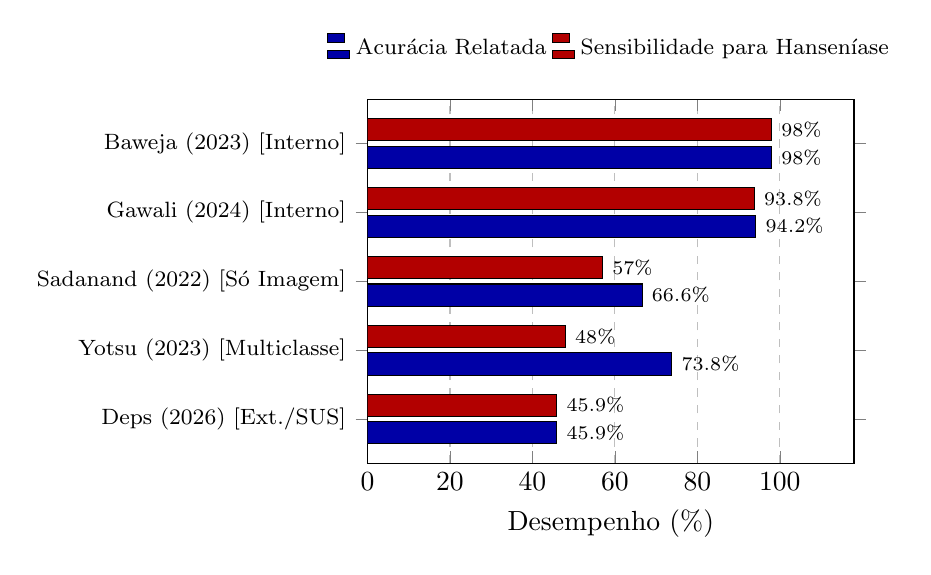
\begin{tikzpicture}
\begin{axis}[
    xbar,
    width=0.64\textwidth,
    height=6.2cm,
    xmin=0, xmax=118,
    xlabel={Desempenho (\%)},
    symbolic y coords={
        {Deps (2026) [Ext./SUS]},
        {Yotsu (2023) [Multiclasse]},
        {Sadanand (2022) [Só Imagem]},
        {Gawali (2024) [Interno]},
        {Baweja (2023) [Interno]}
    },
    ytick=data,
    yticklabel style={font=\footnotesize},
    nodes near coords={\pgfmathprintnumber\pgfplotspointmeta\%},
    nodes near coords align={horizontal},
    every node near coord/.append style={font=\scriptsize},
    bar width=8pt,
    enlarge y limits=0.16,
    xmajorgrids=true,
    grid style=dashed,
    legend style={at={(0.5, 1.08)}, anchor=south, legend columns=2, font=\footnotesize, draw=none}
]
\addplot[fill=blue!65!black, draw=black] coordinates {
    (98.0,{Baweja (2023) [Interno]})
    (94.2,{Gawali (2024) [Interno]})
    (66.6,{Sadanand (2022) [Só Imagem]})
    (73.8,{Yotsu (2023) [Multiclasse]})
    (45.9,{Deps (2026) [Ext./SUS]})
};
\addplot[fill=red!70!black, draw=black] coordinates {
    (98.0,{Baweja (2023) [Interno]})
    (93.8,{Gawali (2024) [Interno]})
    (57.0,{Sadanand (2022) [Só Imagem]})
    (48.0,{Yotsu (2023) [Multiclasse]})
    (45.9,{Deps (2026) [Ext./SUS]})
};
\legend{Acurácia Relatada, Sensibilidade para Hanseníase}
\end{axis}
\end{tikzpicture}
\fonte{Autores.}
\end{figure}

\subsection{Como o desempenho varia entre grupos ou tons de pele?}
\label{subsec:rq5-rq6-tom-pele}

As questões relativas à caracterização do tom de pele (RQ5) e à comparação de desempenho
entre diferentes fototipos cutâneos (RQ6) constituem o núcleo investigativo central deste
trabalho. A síntese dos 25 estudos incluídos revela uma lacuna empírica crítica na literatura
internacional: a quase total ausência de padronização métrica e a inexistência de auditorias
de equidade algorítmica voltadas à hanseníase.

No que tange à caracterização do tom de pele (RQ5), constata-se que a maioria expressiva dos
estudos primários (92\%) omite o uso de escalas dermatológicas validadas, como a classificação
de fototipos de Fitzpatrick (tipos I a VI) ou o ângulo tipológico individual (ITA°). É frequente
o recurso à inferência geográfica indireta, na qual os autores presumem características de
pigmentação a partir do país de recrutamento (como coletas na Índia, Costa do Marfim ou Camarões)
\cite{yotsu2023,barbieri2022}. Nos estudos brasileiros, como \textit{AI4Leprosy} \cite{sadanand2022}
e na base da UFES \cite{deps2026}, registra-se que a heterogeneidade da população nacional
assegurou diversidade fenotípica na amostra; contudo, nenhum dos dois bancos de dados associa
rótulos individuais de fototipo aos metadados públicos de cada fotografia. A única exceção que
relata proporções explícitas é a descrição do aplicativo da OMS \cite{yotsu2026}, que categorizou
as imagens de treino em peles claras (4\%), intermediárias (36\%) e escuras (60\%).

Quanto à variação do desempenho algorítmico entre tons de pele (RQ6), a revisão identificou
um cenário de omissão quase unânime: em 24 dos 25 estudos analisados, não foi reportada nenhuma
métrica de acurácia, sensibilidade ou erro estratificada por fototipo cutâneo. Mesmo no estudo
da OMS \cite{yotsu2026}, onde o tom foi categorizado na base de treinamento, os autores abstiveram-se
de publicar os resultados desagregados por grupo fenotípico.

Esse vácuo de evidências empíricas contrasta com os alertas teóricos reportados em revisões
de inteligência artificial explicável e saúde global \cite{innocent2026,yotsu2025}, que apontam
que redes neurais treinadas predominantemente em repositórios eurocêntricos apresentam viés
sistemático e perdas expressivas de sensibilidade em peles com maior concentração de melanina
(fototipos IV a VI). Em doenças que cursam com manchas hipocrômicas ou placas eritematosas,
a leitura de contraste entre a lesão e o tecido perilesional sádio altera-se drasticamente em
função da pigmentação basal do paciente. A ausência de validação estratificada impede assegurar
que os sistemas computacionais atuais operem de forma justa e segura na rede pública de saúde
do Brasil, justificando a urgência de protocolos de avaliação equitativos no SUS. A
Figura~\ref{fig:vazio-tom-pele} resume o vazio metodológico diagnosticado pela revisão sistemática
tanto na documentação formal de fototipos quanto no cálculo de métricas desagregadas por cor de pele.

\begin{figure}[htbp]
\centering
\caption{Omissão metodológica na caracterização de fototipo (RQ5) e na avaliação de desempenho estratificada (RQ6)}
\label{fig:vazio-tom-pele}
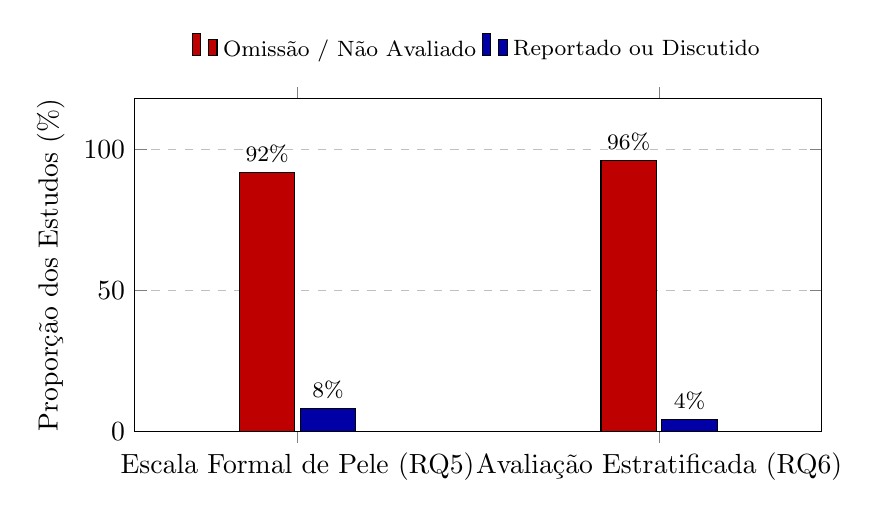
\begin{tikzpicture}
\begin{axis}[
    ybar,
    width=0.85\textwidth,
    height=5.8cm,
    ymin=0, ymax=118,
    ylabel={Proporção dos Estudos (\%)},
    symbolic x coords={
        {Escala Formal de Pele (RQ5)},
        {Avaliação Estratificada (RQ6)}
    },
    xtick=data,
    nodes near coords={\pgfmathprintnumber\pgfplotspointmeta\%},
    nodes near coords align={vertical},
    every node near coord/.append style={font=\footnotesize},
    bar width=20pt,
    enlarge x limits=0.45,
    ymajorgrids=true,
    grid style=dashed,
    legend style={at={(0.5, 1.08)}, anchor=south, legend columns=2, font=\footnotesize, draw=none}
]
\addplot[fill=red!75!black, draw=black] coordinates {
    ({Escala Formal de Pele (RQ5)}, 92)
    ({Avaliação Estratificada (RQ6)}, 96)
};
\addplot[fill=blue!65!black, draw=black] coordinates {
    ({Escala Formal de Pele (RQ5)}, 8)
    ({Avaliação Estratificada (RQ6)}, 4)
};
\legend{Omissão / Não Avaliado, Reportado ou Discutido}
\end{axis}
\end{tikzpicture}
\fonte{Autores.}
\end{figure}

\subsection{Quais modelos e abordagens de inteligência artificial são empregados?}

A análise qualitativa e quantitativa dos 25 estudos incluídos revela uma expressiva evolução metodológica nas arquiteturas computacionais aplicadas ao enfrentamento da hanseníase e demais dermatoses negligenciadas. Em vez de uma única solução hegemônica, identifica-se a coexistência de abordagens clássicas de aprendizado de máquina supervisionado e arquiteturas profundas de ponta, categorizadas em seis grandes famílias:

\begin{enumerate}
    \item \textbf{Redes Neurais Convolucionais Profundas com Transferência de Aprendizado:} Constituem a espinha dorsal da maioria dos estudos de classificação baseados em fotografias clínicas. Destacam-se a ResNet-50 \cite{barbieri2022,yotsu2023,eita2025}, a VGG-16 \cite{yotsu2023,gawali2024}, a Inception-v4 \cite{barbieri2022} e a DenseNet-121 \cite{yotsu2026}. No projeto global da Organização Mundial da Saúde (\textit{WHO Skin NTDs App}), a DenseNet-121 pré-treinada atua em um esquema hierárquico em cascata de dois estágios: o primeiro discrimina se a imagem corresponde a uma dermatose negligenciada e o segundo classifica a lesão entre 12 categorias específicas de NTDs cutâneas \cite{yotsu2026,deps2026,sall2025}.

    \item \textbf{Arquiteturas Otimizadas para Dispositivos Periféricos (\textit{Edge Computing} e Aplicações Móveis):} Visando viabilizar a triagem em regiões endêmicas sem conectividade estável com a internet, modelos como MobileNetV2 foram adaptados mediante técnicas de quantização em ponto fixo de 8 bits \cite{jaikishore2021}, reduzindo drasticamente a pegada de memória e permitindo inferência local em microcontroladores e plataformas como Raspberry Pi com baixo consumo energético, conforme também discutido em iniciativas de telemedicina e \textit{mHealth} \cite{souza2021,yotsu2025}.

    \item \textbf{Modelos Dedicados e Aprendizado com Poucos Exemplos (\textit{Few-Shot Learning}):} Para contornar a escassez crônica de dados primários rotulados, foram desenvolvidas arquiteturas sob medida, como a \textit{LeprosyNet} \cite{baweja2023}, baseada em quatro camadas convolucionais com blocos de normalização em lote (\textit{batch normalization}) e otimizador AdamW. Complementarmente, \citeonline{beesetty2023} e \citeonline{gadekar2023} aplicaram redes siamesas com aprendizado por pares e distância de cosseno (\textit{few-shot learning}), demonstrando capacidade preditiva promissora mesmo quando treinadas em coleções clínicas de tamanho muito restrito.

    \item \textbf{Arquiteturas de Segmentação Semântica e Mecanismos de Atenção:} Para a mensuração objetiva de úlceras plantares e lesões atróficas hansênicas, predominam as redes Fully Convolutional Networks (FCN), U-Net e suas variações com atenção residual (\textit{framework} CO-WinF) \cite{mehta2026}, além da DeepLabV3+ com convoluções atróficas (\textit{atrous convolutions}) para delimitação fina entre tecido epitelial viável, fibrina e leito necrótico \cite{sanchez2024}. Na segmentação baseada em agrupamento adaptativo, \citeonline{jitendra2024heuristic} integraram algoritmos de \textit{Fuzzy C-Means} otimizados pelo algoritmo do vaga-lume (\textit{Firefly Algorithm}).

    \item \textbf{Modelos Clássicos e Otimização Heurística:} Máquinas de Vetores de Suporte (SVM) combinadas com algoritmos de otimização bioinspirados, como o algoritmo do Buraco Negro (\textit{Black Hole Algorithm}) \cite{nyatte2022}, Random Forest e XGBoost continuam sendo empregados com sucesso em conjuntos de dados tabulares, descritores histopatológicos de biópsias \cite{vargasclavijo2025} e na extração combinada de atributos texturais manuais com LBP (\textit{Local Binary Patterns}) e WLD (\textit{Weber Local Descriptor}) \cite{banerjee2023}.

    \item \textbf{Modelos Multimodais e Inteligência Artificial Confiável (\textit{Explainable and Bayesian AI}):} Reconhecendo os limites do diagnóstico estritamente visual, a iniciativa AI4Leprosy \cite{barbieri2022,sadanand2022} desenvolveu modelos híbridos que combinam extratores convolucionais profundos com regressores logísticos penalizados (\textit{elastic-net}) alimentados por variáveis clínicas e anamnese do paciente. Adicionalmente, abordagens bayesianas com \textit{Monte Carlo Dropout} e mapas de saliência visual Grad-CAM foram introduzidas por \citeonline{eita2025} e \citeonline{innocent2026} para mensurar o grau de incerteza da predição e fornecer interpretabilidade às decisões do algoritmo em suporte a profissionais de saúde.
\end{enumerate}

A Figura~\ref{fig:pie-modelos} resume visualmente a distribuição proporcional das famílias e abordagens de inteligência artificial identificadas entre os 25 estudos analisados, evidenciando a predominância de modelos de aprendizagem profunda baseados em convoluções.

\begin{figure}[htbp]
\centering
\caption{Distribuição proporcional das famílias de modelos de inteligência artificial nos 25 estudos}
\label{fig:pie-modelos}
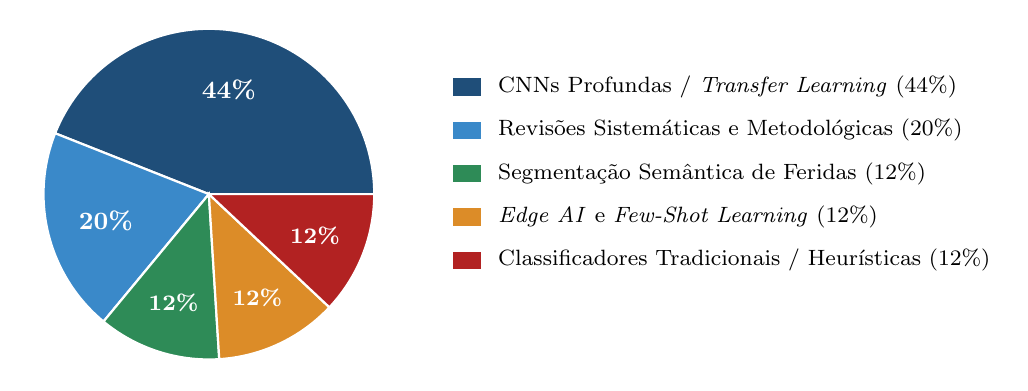
\begin{tikzpicture}
  \definecolor{corCNN}{RGB}{31, 78, 121}
  \definecolor{corRev}{RGB}{58, 137, 201}
  \definecolor{corSeg}{RGB}{46, 139, 87}
  \definecolor{corEdge}{RGB}{220, 140, 40}
  \definecolor{corTrad}{RGB}{178, 34, 34}

  % Slices: 44% (158.4 deg), 20% (72 deg), 12% (43.2 deg), 12% (43.2 deg), 12% (43.2 deg)
  \begin{scope}[shift={(-2.8, 0)}]
    \filldraw[fill=corCNN, draw=white, thick] (0,0) -- (0:2.1) arc (0:158.4:2.1) -- cycle;
    \filldraw[fill=corRev, draw=white, thick] (0,0) -- (158.4:2.1) arc (158.4:230.4:2.1) -- cycle;
    \filldraw[fill=corSeg, draw=white, thick] (0,0) -- (230.4:2.1) arc (230.4:273.6:2.1) -- cycle;
    \filldraw[fill=corEdge, draw=white, thick] (0,0) -- (273.6:2.1) arc (273.6:316.8:2.1) -- cycle;
    \filldraw[fill=corTrad, draw=white, thick] (0,0) -- (316.8:2.1) arc (316.8:360:2.1) -- cycle;

    % Percentagens limpas e legíveis dentro de cada fatia
    \node at (79.2:1.35) [text=white, font=\bfseries\small] {44\%};
    \node at (194.4:1.35) [text=white, font=\bfseries\small] {20\%};
    \node at (252:1.45) [text=white, font=\bfseries\footnotesize] {12\%};
    \node at (295.2:1.45) [text=white, font=\bfseries\footnotesize] {12\%};
    \node at (338.4:1.45) [text=white, font=\bfseries\footnotesize] {12\%};
  \end{scope}

  % Legenda externa limpa e perfeitamente legível à direita
  \begin{scope}[shift={(0.3, 1.25)}]
    \fill[corCNN] (0, 0) rectangle (0.35, 0.22);
    \node[right, font=\footnotesize] at (0.45, 0.11) {CNNs Profundas / \textit{Transfer Learning} (44\%)};

    \fill[corRev] (0, -0.55) rectangle (0.35, -0.33);
    \node[right, font=\footnotesize] at (0.45, -0.44) {Revisões Sistemáticas e Metodológicas (20\%)};

    \fill[corSeg] (0, -1.10) rectangle (0.35, -0.88);
    \node[right, font=\footnotesize] at (0.45, -0.99) {Segmentação Semântica de Feridas (12\%)};

    \fill[corEdge] (0, -1.65) rectangle (0.35, -1.43);
    \node[right, font=\footnotesize] at (0.45, -1.54) {\textit{Edge AI} e \textit{Few-Shot Learning} (12\%)};

    \fill[corTrad] (0, -2.20) rectangle (0.35, -1.98);
    \node[right, font=\footnotesize] at (0.45, -2.09) {Classificadores Tradicionais / Heurísticas (12\%)};
  \end{scope}
\end{tikzpicture}
\fonte{Autores.}
\end{figure}

\subsection{Como a generalização dos modelos é avaliada?}

A avaliação crítica da generalização dos modelos representa um dos achados mais determinantes da presente revisão sistemática, evidenciando uma lacuna estrutural entre os desempenhos computacionais reportados em laboratório e a capacidade real de implantação clínica no Sistema Único de Saúde (SUS):

\begin{enumerate}
    \item \textbf{Hegemonia de Avaliações Monocêntricas e Internas:} Em mais de 90\% dos estudos primários avaliados \cite{banerjee2023,baweja2023,gawali2024,jitendra2024heuristic,vargasclavijo2025}, a validação dos modelos é conduzida unicamente por divisões internas da mesma base de dados (\textit{holdout} ou validação cruzada \textit{k-fold}). Nesses experimentos, as amostras de treino e teste partilham idênticos sensores de captura fotográfica, protocolos institucionais de iluminação e características demográficas de um único centro ou de raspagens da web, mascarando eventuais fragilidades de sobreajuste (\textit{overfitting}).

    \item \textbf{Vazamento de Dados por Falta de Separação Estrita por Paciente:} Conforme apontado criticamente pelas revisões sistemáticas de \citeonline{fernandes2024} e \citeonline{andrade2025}, grande parte dos trabalhos realiza a partição aleatória no nível de imagem (\textit{image-level split}) em vez de garantir uma separação estrita por paciente (\textit{patient-level split}). Quando imagens de diferentes ângulos ou aproximações da mesma lesão pertencem simultaneamente aos conjuntos de treinamento e teste, o modelo decora artefatos de fundo e texturas superficiais do indivíduo, inflando artificialmente as métricas de acurácia.

    \item \textbf{O Fenômeno do Colapso de Domínio na Validação Externa Independente:} O único teste cego, independente e interpopulacional reportado nos estudos incluídos foi conduzido por \citeonline{deps2026} no ambulatório de referência da Universidade Federal do Espírito Santo (UFES). Ao submeter 423 casos reais brasileiros de hanseníase confirmados clínica e histologicamente ao aplicativo da Organização Mundial da Saúde treinado na Europa e África Ocidental \cite{yotsu2026}, o classificador alcançou apenas 45,9\% de sensibilidade Top-1 e 80\% de precisão no Top-3. Mais de metade dos casos de hanseníase foi confundida pelo modelo com outras enfermidades tropicais, como leishmaniose tegumentar e micetoma, evidenciando uma acentuada perda de sensibilidade frente a novas variantes demográficas e fotográficas.

    \item \textbf{A Dependência Crítica da Informação Multimodal:} Os achados de \citeonline{barbieri2022} e \citeonline{sadanand2022} comprovam empiricamente que a generalização puramente fotográfica possui um teto de desempenho intrínseco devido à diversidade morfológica da hanseníase (manchas hipocrômicas, placas infiltradas e tubérculos). A acurácia do modelo saltou de 66,6\% quando alimentado apenas por imagens para 90,0\% quando integrado com metadados clínicos (tempo de evolução da lesão, perda de sensibilidade tátil e térmica e localização anatômica), demonstrando que a capacidade de generalização segura na atenção primária exige integração com o histórico do paciente.

    \item \textbf{Ausência de Ensaios Clínicos Prospectivos:} A totalidade dos estudos de classificação realizou avaliações retrospectivas em bancos de imagens estáticas pré-coletadas. A literatura apenas começa a transitar para estudos de viabilidade prospectivos em cenários comunitários reais de campo, com o delineamento de protocolos clínicos formais como o proposto por \citeonline{sall2025} no Senegal.
\end{enumerate}

A Figura~\ref{fig:tipos-validacao} ilustra a distribuição dos 25 estudos incluídos quanto à abordagem de validação empregada, ressaltando o predomínio esmagador de avaliações fechadas em centros únicos e a raridade de testes externos independentes.

\begin{figure}[htbp]
\centering
\caption{Distribuição dos 25 estudos por abordagem de validação do modelo}
\label{fig:tipos-validacao}
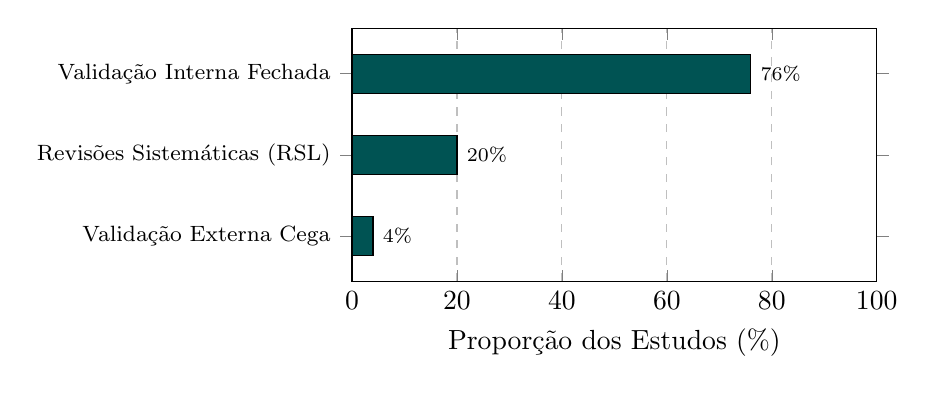
\begin{tikzpicture}
\begin{axis}[
    xbar,
    width=0.68\textwidth,
    height=4.8cm,
    xmin=0, xmax=100,
    xlabel={Proporção dos Estudos (\%)},
    symbolic y coords={
        {Validação Externa Cega},
        {Revisões Sistemáticas (RSL)},
        {Validação Interna Fechada}
    },
    ytick=data,
    yticklabel style={font=\footnotesize},
    nodes near coords={\pgfmathprintnumber\pgfplotspointmeta\%},
    nodes near coords align={horizontal},
    every node near coord/.append style={font=\scriptsize},
    bar width=14pt,
    enlarge y limits=0.28,
    xmajorgrids=true,
    grid style=dashed
]
\addplot[fill=teal!65!black, draw=black] coordinates {
    (76.0,{Validação Interna Fechada})
    (20.0,{Revisões Sistemáticas (RSL)})
    (4.0,{Validação Externa Cega})
};
\end{axis}
\end{tikzpicture}
\fonte{Autores.}
\end{figure}

\subsection{Em quais veículos os estudos são publicados?}

A distribuição dos 25 estudos incluídos quanto ao veículo de disseminação científica evidencia uma clara preponderância de periódicos indexados de alto fator de impacto sobre anais de congressos, além de demonstrar um notável caráter interdisciplinar entre as ciências da computação, a dermatologia e a saúde pública global:

\begin{itemize}
    \item \textbf{Periódicos Científicos (\textit{Journals}):} Totalizam 20 dos 25 estudos selecionados (80,0\% do corpo amostral). Essa concentração reflete o amadurecimento científico da temática e a necessidade de validação metodológica rigorosa por pares. Entre os periódicos da área médica, dermatológica e de saúde pública internacional, incluem-se veículos de prestígio como \textit{The Lancet Regional Health -- Americas} \cite{barbieri2022,sadanand2022}, \textit{PLOS Neglected Tropical Diseases} \cite{yotsu2023}, \textit{Revista Panamericana de Salud Pública} \cite{deps2026}, \textit{Journal of Investigative Dermatology} \cite{yotsu2026}, \textit{International Health} \cite{yotsu2025}, \textit{Frontiers in Medicine} \cite{deps2024}, \textit{The American Journal of Dermatopathology} \cite{vargasclavijo2025}, \textit{Indian Journal of Leprosy} \cite{beesetty2023}, \textit{Portuguese Journal of Dermatology and Venereology} \cite{goswami2026}, \textit{Journal of Clinical Medicine} \cite{fernandes2024}, \textit{JMIR Research Protocols} \cite{sall2025} e \textit{Malahayati International Journal of Nursing and Health Science} \cite{prayitno2026}. No domínio da computação aplicada e bioinformática médica, destacam-se \textit{PLOS Computational Biology} \cite{andrade2025}, \textit{Engineering Applications of Artificial Intelligence} \cite{eita2025}, \textit{BMC Artificial Intelligence} \cite{innocent2026}, \textit{Informatics in Medicine Unlocked} \cite{nyatte2022}, \textit{SN Computer Science} \cite{banerjee2023,jitendra2024heuristic} e \textit{The International Journal of Lower Extremity Wounds} \cite{mehta2026}.

    \item \textbf{Anais de Conferências Internacionais (\textit{Conference Proceedings}):} Correspondem aos 5 estudos restantes (20,0\% da seleção), congregando trabalhos focados no desenvolvimento experimental rápido de novos modelos, segmentação de imagem e soluções de \textit{hardware} embarcado para a atenção periférica. Destacam-se eventos chancelados pelo IEEE: \textit{IEEE International Conference on Image Processing} (ICIP) \cite{sanchez2024}, \textit{IEEE India Council International Conference} (INDICON) \cite{jaikishore2021}, \textit{IEEE International Conference on Computing, Communication and Networking Technologies} (ICCCNT) \cite{gawali2024}, \textit{IEEE International Conference on Emerging Trends in Computing and Communication} (ETCOM) \cite{ahikpa2025} e a \textit{International Conference on Sustainable Computing and Data Communication Systems} (ICSCDS) \cite{baweja2023}.
\end{itemize}

A evolução temporal dos veículos demonstra uma relevante mudança de paradigma: enquanto os estudos pioneiros (2021--2023) concentravam-se em anais de conferências de computação focados na viabilidade técnica exploratória de classificadores em pequenas amostras, as publicações entre 2024 e 2026 migraram expressivamente para periódicos médicos e de saúde coletiva. Esse movimento assinala que a pesquisa sobre visão computacional em hanseníase ultrapassou a fase restrita de experimentação em bancada e ingressou definitivamente na discussão sobre validação clínica independente, explicabilidade algorítmica, equidade diagnóstica e integração operacional aos sistemas de saúde pública. A Figura~\ref{fig:veiculos-evolucao} ilustra a trajetória ascendente das publicações ao longo dos anos e a consolidação dos periódicos indexados como principal canal de divulgação científica da área.

\begin{figure}[htbp]
\centering
\caption{Evolução temporal e distribuição dos 25 estudos por tipo de veículo de publicação (2021--2026)}
\label{fig:veiculos-evolucao}
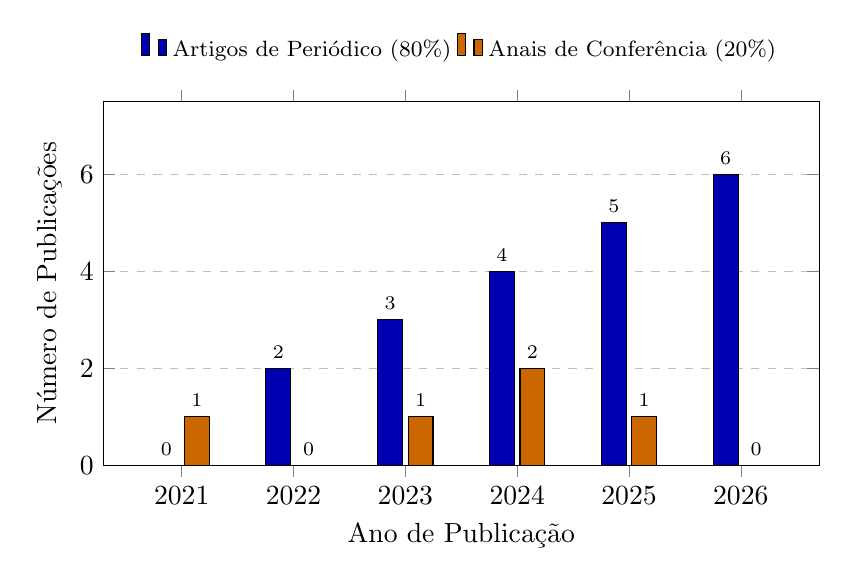
\begin{tikzpicture}
\begin{axis}[
    ybar,
    width=0.88\textwidth,
    height=6.2cm,
    ymin=0, ymax=7.5,
    ylabel={Número de Publicações},
    xlabel={Ano de Publicação},
    symbolic x coords={2021, 2022, 2023, 2024, 2025, 2026},
    xtick=data,
    nodes near coords,
    every node near coord/.append style={font=\scriptsize},
    bar width=9pt,
    enlarge x limits=0.14,
    ymajorgrids=true,
    grid style=dashed,
    legend style={at={(0.5, 1.08)}, anchor=south, legend columns=2, font=\footnotesize, draw=none}
]
\addplot[fill=blue!70!black, draw=black] coordinates {
    (2021, 0)
    (2022, 2)
    (2023, 3)
    (2024, 4)
    (2025, 5)
    (2026, 6)
};
\addplot[fill=orange!80!black, draw=black] coordinates {
    (2021, 1)
    (2022, 0)
    (2023, 1)
    (2024, 2)
    (2025, 1)
    (2026, 0)
};
\legend{Artigos de Periódico (80\%), Anais de Conferência (20\%)}
\end{axis}
\end{tikzpicture}
\fonte{Autores.}
\end{figure}
